\section{猜數字:幾A幾B(電腦猜)}

使用者選定一個沒有重複的三位數當作答案,電腦每猜一個數字,使用者就要根據答案給出幾A幾B的提示。A表示位置正確的數的個數,B表示數字正確但位置錯誤的數的個數。

電腦根據提示一直猜,直到猜中為止。
\begin{figure}[H]
	\centering
	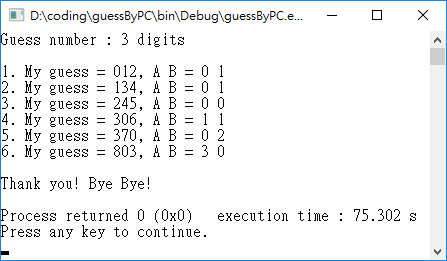
\includegraphics{fig/PC}
\end{figure}
\subsection{解題思惟}

\subsubsection{程式流程:}
\begin{enumerate}
	\item 初始化陣列,將不可能成為答案的元素設成0,其他設成1。
	\item 輸出一個可能的答案。
	\item 讓使用者輸入幾A幾B。
	\item 根據幾A幾B將不可能的答案剔除。
	\item 若沒猜中,回到步驟2,猜中則結束程式。
\end{enumerate}

\subsubsection{函式說明:}
\begin{enumerate}
	\item void initCandidates()
	
	此函數用來初始化陣列。在0-999的整數中,分別取出個位、十位及百位數。若三個數字有重複,則不可能成為答案,將此元素設為0,其他元素設為1。
	
	\item int validGuess()
	
	此函數選出電腦猜的數字。用for迴圈掃描陣列,若是可能的答案,則回傳。
	
	\item updateCandidates(int number, int ga, int gb)
	
	此函數用來更新陣列。用for迴圈掃描陣列,若是可能的答案,判斷是否符合幾A幾B,若不符合,則將此元素設為0。
\end{enumerate}

\subsection{程式碼}
\begin{cppcode}
#include <cstdio>

int candidates[1000];

void initCandidates();
int  validGuess();
void updateCandidates(int number, int ga, int gb);
int  countA(int guess, int ans);
int  countB(int guess, int ans);

int main()
{
	int guess, idx=1, a, b;
	
	initCandidates();
	printf("Guess number : 3 digits\n\n");
	do {
		guess = validGuess();
		printf("%d. My guess = %03d, A B = ", idx++, guess);
		scanf("%d%d", &a, &b);
		updateCandidates(guess, a, b);
	} while (a!=3 || b!=0);
	printf("\nThank you! Bye Bye!\n");
	
	return 0;
}

// init candidates, erase all number with same digit
void initCandidates()
{
	for (int n=0; n<1000; n++) {
		int a = n/100;       // a..
		int b = (n/10) % 10; // .b.
		int c = n % 10;      // ..c
		if (a==b || b==c || c==a) candidates[n]=0;
		else candidates[n]=1;
	}
}

int validGuess()
{
	for (int i=0; i<1000; i++) {
		if (candidates[i]) return i;
	}
	return -1; // No possible candidate
}

void updateCandidates(int number, int ga, int gb)
{
	for (int i=0; i<1000; i++) {
		if (candidates[i]) {
			if (ga != countA(number, i)) candidates[i] = 0;
			if (gb != countB(number, i)) candidates[i] = 0;
		}
	}
}

int countA(int guess, int ans)
{
	int d1, d2, cnt=0;
	for (int i=0; i<3; i++) {
		d1 = guess % 10;
		d2 = ans % 10;
		if (d1==d2) cnt++;
		guess /= 10;
		ans /= 10;
	}
	return cnt;
}

int countB(int guess, int ans)
{
	int a[3], b[3], cnt=0;
	for (int i=0; i<3; i++) {
		a[i] = guess % 10;
		b[i] = ans % 10;
		guess /= 10;
		ans /= 10;
	}
	for (int i=0; i<3; i++) {
		for (int j=0; j<3; j++) {
			if (i!=j && a[i]==b[j]) cnt++;
		}
	}
	return cnt;
}

\end{cppcode}